%==============================================================================
%  MATH 231 -- Applied Linear Algebra (Queens College, Fall 2026)
%  LECTURE 1 -- Tuesday, September 1, 2026 -- Kiely Hall 326, 12:10-2:00 PM
%
%  Section 1: "Vectors: Magnitude, Direction, the Norm, and Addition"
%
%  STATUS: in progress.  This document currently contains the FIRST content
%  section of Lecture 1 only; further sections will be appended below the
%  practice set as the lecture is built out.
%
%  Conventions used in this file:
%     \inote{...}   -- instructor note: NOT board content, planning only
%     \board{...}   -- an explicit board / drawing cue
%     \tchip{...}   -- the time budget for the section it sits beside
%  Timing rationale and the lean/full variants are in "Timing" at the end.
%
%  Compile with pdflatex (standard TeX Live packages only; uses tikz).
%==============================================================================
\documentclass[11pt]{article}

\usepackage[margin=1in]{geometry}
\usepackage{amsmath,amssymb,amsthm}
\usepackage[dvipsnames]{xcolor}
\usepackage{enumitem}
\usepackage{booktabs}
\usepackage{array}
\usepackage[hidelinks]{hyperref}
\usepackage{titlesec}
\usepackage{needspace}
\usepackage{tikz}
\usetikzlibrary{arrows.meta}

%------------------------------------------------------------------ style ----
\titleformat{\section}{\large\bfseries\sffamily}{\thesection.}{0.6em}{}
\titleformat{\subsection}{\normalsize\bfseries\sffamily}{\thesubsection.}{0.5em}{}
\titlespacing*{\section}{0pt}{14pt}{6pt}

\newcommand{\tchip}[1]{{\normalfont\small\sffamily\bfseries
  \colorbox{RoyalBlue!12}{\strut\,#1\,}}}

\newcommand{\inote}[1]{\par\smallskip\noindent
  {\small\sffamily\color{black!65}%
   \textbf{\textcolor{RoyalBlue}{Instructor note.}}\ #1}\par\smallskip}

\newcommand{\board}[1]{\par\smallskip\noindent
  {\small\sffamily\color{black!70}%
   \textbf{\textcolor{ForestGreen}{At the board.}}\ #1}\par\smallskip}

\theoremstyle{definition}
\newtheorem{defn}{Definition}
\newtheorem{ex}{Example}
\theoremstyle{remark}
\newtheorem*{rmk}{Remark}

% Forward-reference flags, in the spirit of the "honest forward references"
% named in the course-progression document.
\newcommand{\lookahead}{\par\smallskip\noindent
  \textbf{\sffamily\textcolor{RoyalBlue}{Looking ahead.}}\ \ignorespaces}
\newcommand{\lookaheadt}[1]{\par\smallskip\noindent
  \textbf{\sffamily\textcolor{RoyalBlue}{Looking ahead --- #1}}\ \ignorespaces}

%--------------------------------------------------------------- notation ----
\newcommand{\R}{\mathbb{R}}
\newcommand{\vc}[1]{\mathbf{#1}}
\newcommand{\norm}[1]{\lVert #1\rVert}

%------------------------------------------------------------- tikz helpers --
\tikzset{
  vecarr/.style   = {-{Stealth[length=2.6mm,width=2.0mm]},very thick},
  thinarr/.style  = {-{Stealth[length=2.2mm,width=1.7mm]},thick},
  axisline/.style = {->,gray!75,thin}
}
% \lattice{xmin}{xmax}{ymin}{ymax}
\newcommand{\lattice}[4]{%
  \draw[step=1cm,gray!25,very thin] (#1,#3) grid (#2,#4);
  \draw[axisline] (#1,0) -- (#2+0.45,0) node[right,font=\scriptsize,black]{$x$};
  \draw[axisline] (0,#3) -- (0,#4+0.45) node[above,font=\scriptsize,black]{$y$};
}

\title{\vspace{-1.2cm}\textbf{\sffamily MATH 231 -- Applied Linear Algebra}\\[4pt]
       {\large\sffamily Lecture 1 \textbullet\ Vectors: Magnitude, Direction,
        the Norm, and Addition}\\[2pt]
       {\normalsize\sffamily Tuesday, September 1, 2026 \textbullet\
        Kiely Hall 326 \textbullet\ Instructor: Kevin Bedoya}}
\author{}
\date{\normalsize\sffamily Draft dated August 23, 2026}

\begin{document}
\maketitle
\vspace{-1.1cm}

%==============================================================================
\section*{Session plan}
%==============================================================================
\noindent
\begin{tabular}{@{}r l l@{}}
\toprule
\textbf{\S} & \textbf{Segment} & \textbf{Budget} \\
\midrule
0 & Syllabus, logistics, course introduction            & 25 min \\
1 & Vectors: magnitude, direction, the Euclidean plane  &  8 min \\
2 & The norm --- our first vector operation             &  7 min \\
3 & Bridge to calculus: the derivative as a vector      &  6 min \\
4 & Vector quantities vs.\ scalar quantities            &  4 min \\
5 & One-dimensional vectors                             &  3 min \\
6 & Notation and set-theoretic placement                &  5 min \\
7 & Addition and subtraction                            &  7 min \\
8 & Practice set P1--P4                                 & 15 min \\
  & Questions / transitions (slack)                     &  5 min \\
\midrule
  & \textbf{Content total (\S1--8)}                      & \textbf{60 min} \\
  & \textbf{Session total}                              & \textbf{85 min} \\
\bottomrule
\end{tabular}

\vspace{6pt}
\noindent\textbf{Learning objectives.} By the end of the session a student can:
state what a vector is in terms of magnitude and direction; identify the tail
and head of a vector in $\R^2$; compute the Euclidean norm of a vector and
explain why it is a \emph{unary} operation; distinguish vector quantities from
scalar quantities; read all three notational conventions for a vector; and add
and subtract vectors in $\R^2$ both componentwise and geometrically.

\inote{Prerequisite reach-back is deliberately shallow --- Pythagoras and the
notion of a derivative are the only things assumed. \S3 is the only segment
that requires calculus, and it is motivational: nothing later in the course
depends on it, so it is the first candidate to trim if the clock demands.}

\lookaheadt{placement in the course progression.} \S1--\S2 and \S6--\S8 belong to
Unit~1 (\emph{Vectors, Vector Spaces \& the Language of the Course}), with one
deliberate forward pull: the Euclidean ($\ell_2$) norm is formally a Unit~2
object, but ``magnitude'' is the natural entry point to a vector, so the
$\ell_2$ norm is introduced here and the general $p$-norm family, the induced
metric, and the inner product are deferred to Unit~2 where they belong.

\medskip
\noindent\textbf{Textbook alignment.}
\textbf{[BV]} Ch.~1 (vectors, addition, scalar multiplication), Ch.~3 (norm and
distance); \textbf{[S]} Ch.~1; \textbf{[A]} Ch.~1; \textbf{[TB]} Lec.~2--3
(norms).

%==============================================================================
\section[Vectors: magnitude, direction, and the space they live in]%
        {Vectors: magnitude, direction, and the space they live in
         \hfill \tchip{8 min}}
%==============================================================================
We begin with a working definition --- deliberately informal, and stated in the
language of quantities rather than axioms.

\begin{defn}[Vector, working definition]
A \emph{vector} is a mathematical object carrying two attributes:
a \textbf{magnitude} and a \textbf{direction}.
\end{defn}

\lookahead This is the physicist's definition, and it is the right one to start
from because it is the one you can \emph{see}. Later in the course we replace it
with the algebraist's definition: a vector will become any element of a set
equipped with two operations obeying a short list of axioms --- at which point
functions, polynomials, and matrices all become vectors too, and ``magnitude and
direction'' stops being the defining feature. For now, hold on to the picture.

\subsection*{The space a vector lives in}
A vector does not exist in isolation; it lives in a space. Ours today is the
\textbf{two-dimensional Euclidean plane}, the familiar $xy$-plane, and every
vector we draw will live in it.

The word \emph{dimension} here means a \textbf{degree of freedom} with respect
to spatial coordinates: how many independent numbers must you supply to pin down
a location? On a line, one; on the plane, two --- an $x$ and a $y$, chosen
independently of one another. The plane is two-dimensional in exactly that
sense.

\subsection*{Tail, head, and the two attributes}
Fix the point $(1,2)$. Draw an arrow from the origin to it. That arrow is a
vector, and it has two distinguished points:

\begin{itemize}[leftmargin=1.4em,itemsep=2pt]
  \item the \textbf{tail} --- where the arrow begins, here the origin $(0,0)$;
  \item the \textbf{head} --- where the arrow ends and the arrowhead is drawn,
        here $(1,2)$.
\end{itemize}

\noindent With the tail and head named, the two attributes become concrete:

\begin{itemize}[leftmargin=1.4em,itemsep=2pt]
  \item \textbf{Direction} is the arrow's orientation in the plane --- which way
        it points, relative to the axes, as it travels from tail to head. The
        arrow to $(1,2)$ points up and to the right, more steeply up than
        rightward.
  \item \textbf{Magnitude} is the arrow's \textbf{length}: the distance from the
        tail to the head. We measure it with the Euclidean distance, and we
        compute it in \S2.
\end{itemize}

\board{Draw the left-hand figure only. Mark the tail, mark the head, draw the
arrowhead conspicuously --- the arrowhead \emph{is} the direction, and students
who draw bare line segments lose that information.}

\begin{center}
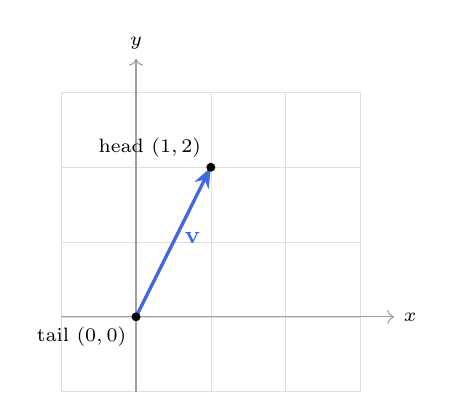
\begin{tikzpicture}[scale=0.95]
  \lattice{-1}{3}{-1}{3}
  \draw[vecarr,RoyalBlue] (0,0) -- (1,2);
  \fill (0,0) circle (1.7pt);
  \fill (1,2) circle (1.7pt);
  \node[below left,font=\scriptsize]  at (0,0) {tail $(0,0)$};
  \node[above left,font=\scriptsize]  at (1,2) {head $(1,2)$};
  \node[right,font=\small,RoyalBlue]  at (0.52,1.05) {$\vc{v}$};
\end{tikzpicture}
\hspace{1.4cm}
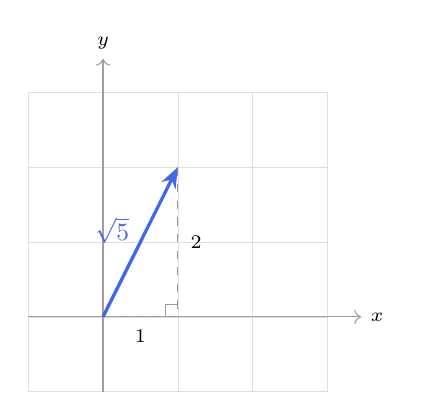
\begin{tikzpicture}[scale=0.95]
  \lattice{-1}{3}{-1}{3}
  \draw[dashed,gray!80] (0,0) -- (1,0) -- (1,2);
  \draw[gray!80] (0.84,0) -- (0.84,0.16) -- (1,0.16);
  \draw[vecarr,RoyalBlue] (0,0) -- (1,2);
  \node[below,font=\scriptsize] at (0.5,-0.04) {$1$};
  \node[right,font=\scriptsize] at (1.04,1) {$2$};
  \node[left,font=\small,RoyalBlue] at (0.48,1.15) {$\sqrt{5}$};
\end{tikzpicture}
\end{center}

%==============================================================================
\section[The norm --- our first vector operation]%
        {The norm --- our first vector operation \hfill \tchip{7 min}}
%==============================================================================
The magnitude of a vector is not just a description of it; it is something we
\emph{compute} from it. Computing it is our first vector operation, and it has a
name.

\begin{defn}[Euclidean norm in $\R^2$]
For a vector $\vc{v}$ with tail at the origin and head at $(x,y)$, the
\textbf{Euclidean norm} of $\vc{v}$ is
\[
  \norm{\vc{v}} \;=\; \sqrt{x^{2}+y^{2}},
\]
the Euclidean distance from the tail to the head.
\end{defn}

Two things to notice about the shape of this operation.

\begin{itemize}[leftmargin=1.4em,itemsep=3pt]
  \item It is \textbf{unary}: it takes \emph{one} vector as input. Compare $3+5$,
        where addition consumes two numbers --- a \emph{binary} operation. The
        norm consumes one vector and returns one number.
  \item It maps a \emph{vector} to a \emph{scalar}: $\norm{\cdot}:\R^2\to\R$,
        and the output is never negative. Length cannot be negative.
\end{itemize}

\noindent The formula is Pythagoras, nothing more. The right-hand figure above
is the proof: the horizontal leg has length $x$, the vertical leg has length
$y$, and the vector is the hypotenuse.

\begin{ex}[The running vector]
For $\vc{v}$ with head at $(1,2)$,
\[
  \norm{\vc{v}} \;=\; \sqrt{1^{2}+2^{2}} \;=\; \sqrt{1+4} \;=\; \sqrt{5}
  \;\approx\; 2.236.
\]
\end{ex}

\begin{ex}[A clean one]
For $\vc{w}$ with head at $(3,4)$,
$\norm{\vc{w}}=\sqrt{9+16}=\sqrt{25}=5$.
\end{ex}

\inote{Do $\sqrt5$ first and $(3,4)$ second, in that order. The first example
teaches that a norm is generically irrational and that $\sqrt{5}$ is a finished
answer requiring no decimal; the second is the reward. Reversing them trains
students to expect integers and to distrust radicals.}

\begin{rmk}
So three phrases now name the same number: the \emph{magnitude} of the vector,
the \emph{length} of the arrow, and the \emph{Euclidean norm} $\norm{\vc{v}}$.
Use them interchangeably.
\end{rmk}

\inote{Suppressed on purpose: ``magnitude $=$ norm'' holds \emph{up to the
choice of underlying metric}, and there are other norms --- $\ell_1$,
$\ell_\infty$, the general $p$-norm --- under which the same arrow has a
different length. Do not raise this today; naming a choice students cannot yet
see makes the definition feel arbitrary. It is Unit~2 material, and the
$\ell_1/\ell_\infty$ contrast is the payoff of introducing it there.}

%==============================================================================
\section[Bridge to calculus: the derivative as a vector quantity]%
        {Bridge to calculus: the derivative as a vector quantity
         \hfill \tchip{6 min}}
%==============================================================================
Vectors are not new to you --- you have been computing one all through calculus
without calling it that.

Let $f$ be differentiable and consider the tangent line to the curve $y=f(x)$ at
a point. The tangent line has both of our attributes:

\begin{itemize}[leftmargin=1.4em,itemsep=3pt]
  \item \textbf{Direction.} The \emph{sign} of the slope orients it. A positive
        slope tilts up-and-to-the-right and the function is increasing there; a
        negative slope tilts down-and-to-the-right and the function is
        decreasing. The tangent line points somewhere.
  \item \textbf{Magnitude.} The \emph{size} of the slope measures how fast the
        function is changing --- the ``speed'' of change in that direction. A
        slope of $10$ climbs ten times as urgently as a slope of $1$.
\end{itemize}

\noindent Direction plus magnitude: the derivative of $f$ at a point can be read
as a \textbf{vector quantity}.

Concretely, take $f(x)=x^{2}$ at $x=1$. Then $f'(1)=2$, so from the point
$(1,1)$ the tangent advances $1$ unit rightward for every $2$ units upward: its
direction vector is $[\,1,\,2\,]$ --- the very vector we drew in \S1, now
carrying a meaning. Its norm, $\sqrt{5}$, is the rate at which arc length
accumulates along the tangent per unit of horizontal travel.

\begin{center}
\begin{tikzpicture}[scale=1.05]
  \draw[axisline] (-1.35,0) -- (2.6,0) node[right,font=\scriptsize,black]{$x$};
  \draw[axisline] (0,-1.15) -- (0,4.35) node[above,font=\scriptsize,black]{$y$};
  \draw[BrickRed,thick,domain=-1.15:2.05,smooth,variable=\x]
        plot ({\x},{\x*\x});
  % the tangent y = 2x-1, drawn solid so it reads as a line: the vector below
  % lies ON it and would otherwise hide most of a dashed stroke
  \draw[gray!55,thick] (0.05,-0.9) -- (2.4,3.8);
  \draw[vecarr,RoyalBlue] (1,1) -- (2,3);
  \fill (1,1) circle (1.7pt);
  \node[below right,font=\scriptsize]   at (1.03,0.97) {$(1,1)$};
  \node[right,font=\small,RoyalBlue]    at (1.52,1.92) {$[\,1,\,2\,]$};
  \node[left,font=\scriptsize,BrickRed] at (-1.1,1.45) {$y=x^{2}$};
  \node[right,font=\scriptsize,gray]    at (2.42,3.8) {tangent at $x=1$};
\end{tikzpicture}
\end{center}

%==============================================================================
\section[Vector quantities vs.\ scalar quantities]%
        {Vector quantities vs.\ scalar quantities \hfill \tchip{4 min}}
%==============================================================================
The phrase from \S3 is worth making official, because it sorts most of the
quantities you will meet in the sciences into two bins.

\begin{itemize}[leftmargin=1.4em,itemsep=3pt]
  \item A \textbf{vector quantity} has a magnitude \emph{and} a direction.
        \emph{Examples:} displacement, velocity, acceleration, force, momentum,
        torque, the electric and magnetic fields, a temperature \emph{gradient}.
  \item A \textbf{scalar quantity} has a magnitude only --- it indicates
        \emph{scale}, and nothing else. \emph{Examples:} mass, speed,
        temperature, energy, work, electric charge, time, pressure, density,
        volume.
\end{itemize}

\noindent The pair to dwell on is \textbf{speed} and \textbf{velocity}. Speed is
a scalar: $60$ mph. Velocity is a vector: $60$ mph \emph{due north}. Speed is
exactly the magnitude of the velocity vector --- that is, its norm --- which is
why the two words are not synonyms and why a car going round a bend at constant
speed is nonetheless accelerating.

\inote{This is the segment where students volunteer examples from their own
majors; it can absorb unlimited time. Take two examples, then move on.}

%==============================================================================
\section[One-dimensional vectors]%
        {One-dimensional vectors \hfill \tchip{3 min}}
%==============================================================================
Nothing above required two dimensions. In one dimension --- on the number line
--- a vector is a signed number, and the two attributes are still both present:

\begin{itemize}[leftmargin=1.4em,itemsep=2pt]
  \item the \textbf{sign} carries the direction: positive points one way along
        the line, negative the other;
  \item the \textbf{absolute value} carries the magnitude.
\end{itemize}

% keep this paragraph and the number line it describes on one page
\Needspace*{11\baselineskip}
\noindent So $u=3$ and $w=-3$ have the same magnitude and opposite directions.
And the one-dimensional norm is
$\norm{u}=\sqrt{u^{2}}=\lvert u\rvert$ --- absolute value was your first norm
all along.

\begin{center}
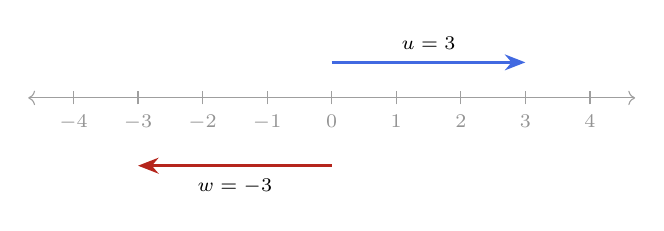
\begin{tikzpicture}[scale=0.82]
  \draw[<->,gray!75,thin] (-4.7,0) -- (4.7,0);
  \foreach \i in {-4,-3,-2,-1,0,1,2,3,4} {
    \draw[gray!75] (\i,-0.1) -- (\i,0.1);
    \node[below,font=\scriptsize,gray!85] at (\i,-0.12) {$\i$};
  }
  \draw[vecarr,RoyalBlue] (0,0.55) -- (3,0.55);
  \node[above,font=\scriptsize] at (1.5,0.6) {$u=3$};
  \draw[vecarr,BrickRed] (0,-1.05) -- (-3,-1.05);
  \node[below,font=\scriptsize] at (-1.5,-1.1) {$w=-3$};
\end{tikzpicture}
\end{center}

%==============================================================================
\section[Notation, and where vectors sit set-theoretically]%
        {Notation, and where vectors sit set-theoretically
         \hfill \tchip{5 min}}
%==============================================================================
There are several standard ways to denote a vector symbolically. Using the
letter $v$ purely as an example --- \emph{any} letter may be used:

\begin{center}
\renewcommand{\arraystretch}{1.35}
\begin{tabular}{@{}c l@{}}
\toprule
\textbf{Notation} & \textbf{Reading} \\
\midrule
$\vc{v}$      & boldface --- common in applied and computational writing \\
$\vec{v}$     & arrow overhead --- common in physics and calculus texts \\
$v$           & plain --- common in pure linear algebra, where context suffices \\
\bottomrule
\end{tabular}
\end{center}

\noindent\textbf{In this class we will use a mixture of all three}, and context
will tell you which object you are looking at. Getting comfortable reading all
three is part of the course: you will meet all of them in the reference texts.

\subsection*{The set-theoretic statement}
To say that $\vc{v}$ is a two-dimensional vector, we write
\[
  \vc{v}\in\R^{2},
  \qquad\text{where}\qquad
  \R^{2}\;=\;\R\times\R\;=\;\bigl\{(x,y)\;:\;x\in\R,\;y\in\R\bigr\}.
\]
Read aloud: ``$\vc{v}$ is in $\R$-two.'' The superscript $2$ is the dimension of
\S1 --- two coordinates, each free to be any real number, chosen independently.

\subsection*{The numerical convention for this class}
We write a vector in brackets, listing its coordinates in order:
\[
  \vc{v}=[\,x,\,y\,],
  \qquad\text{for instance}\qquad
  \vc{v}=[\,1,\,2\,].
\]

\inote{Order matters and will not be belabored again: $[1,2]\neq[2,1]$. Say it
once here.}

\lookahead At this stage of the course, a vector \emph{is} a point of the plane
together with the convention that its tail sits at the origin: the head is
$(x,y)$ and the arrow is drawn from $(0,0)$. This is a temporary simplification
and we will discard it once you are fluent --- a vector is really a
\emph{displacement}, so the same vector may be drawn with its tail anywhere,
which is precisely what makes the head-to-tail picture in \S7 legitimate.

%==============================================================================
\section[Addition and subtraction]%
        {Addition and subtraction \hfill \tchip{7 min}}
%==============================================================================
Many operations on vectors await us. Here are the first two binary ones ---
each consumes \emph{two} vectors and returns a vector, in contrast to the norm
of \S2.

\begin{defn}[Addition and subtraction in $\R^2$]
Let $\vc{u},\vc{v}\in\R^{2}$ with $\vc{u}=[x_1,y_1]$ and $\vc{v}=[x_2,y_2]$.
Then
\[
  \vc{u}+\vc{v}=[\,x_1+x_2,\;\;y_1+y_2\,],
  \qquad
  \vc{u}-\vc{v}=[\,x_1-x_2,\;\;y_1-y_2\,].
\]
\end{defn}

\noindent Both are \textbf{componentwise}: the first coordinates interact only
with each other, and likewise the second. Nothing mixes across slots.

\begin{ex}[Worked at the board]
Let $\vc{u}=[2,1]$ and $\vc{v}=[1,3]$. Then
\[
  \vc{u}+\vc{v}=[\,2+1,\;1+3\,]=[\,3,\,4\,],
  \qquad
  \vc{u}-\vc{v}=[\,2-1,\;1-3\,]=[\,1,\,-2\,].
\]
And since we know how to take a norm: $\norm{\vc{u}+\vc{v}}=\sqrt{9+16}=5$ ---
the clean vector from \S2, arrived at by addition.
\end{ex}

\subsection*{What the pictures say}
\textbf{Addition} is the \emph{parallelogram rule}: place $\vc{u}$ and $\vc{v}$
tail-to-tail at the origin, complete the parallelogram, and $\vc{u}+\vc{v}$ is
the diagonal from the origin. Equivalently --- \emph{head to tail} --- walk
along $\vc{u}$, then from where you land walk along $\vc{v}$; the sum is the
single arrow from start to finish.

\textbf{Subtraction} is addition of the opposite, $\vc{u}-\vc{v}=\vc{u}+(-\vc{v})$,
and it has its own reading: $\vc{u}-\vc{v}$ is the arrow \emph{from the head of
$\vc{v}$ to the head of $\vc{u}$}. It is the displacement that takes you from
$\vc{v}$ to $\vc{u}$, which is why differences of vectors are how we will
measure how far apart two vectors are.

\begin{center}
% both lattices share the same extent so the two pictures align side by side
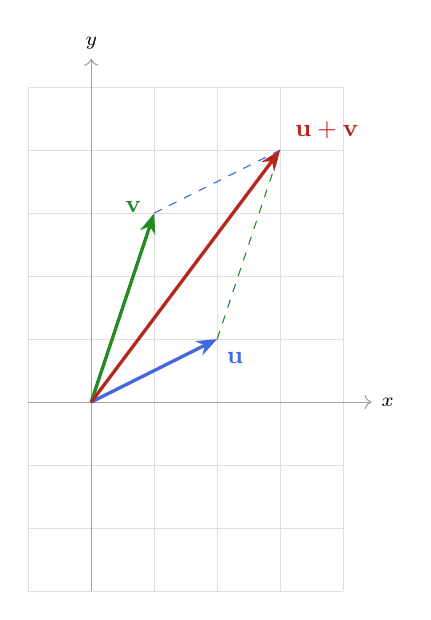
\begin{tikzpicture}[scale=0.8]
  \lattice{-1}{4}{-3}{5}
  \draw[ForestGreen,dashed] (2,1) -- (3,4);
  \draw[RoyalBlue,dashed]   (1,3) -- (3,4);
  \draw[vecarr,RoyalBlue]   (0,0) -- (2,1);
  \draw[vecarr,ForestGreen] (0,0) -- (1,3);
  \draw[vecarr,BrickRed]    (0,0) -- (3,4);
  \node[below right,font=\small,RoyalBlue]  at (2,0.95) {$\vc{u}$};
  \node[left,font=\small,ForestGreen]       at (0.95,3.1) {$\vc{v}$};
  \node[right,font=\small,BrickRed]         at (3.08,4.32) {$\vc{u}+\vc{v}$};
\end{tikzpicture}
\hspace{1.0cm}
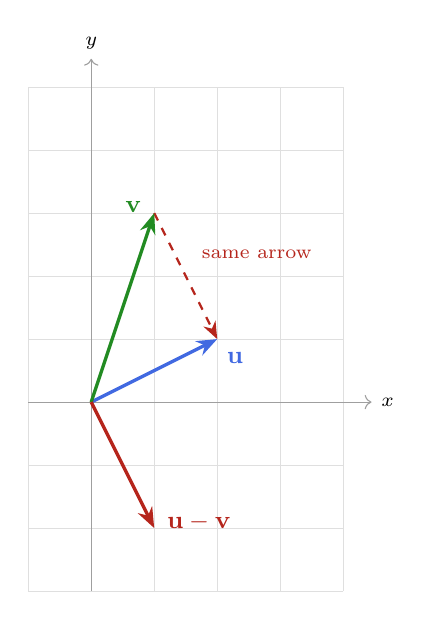
\begin{tikzpicture}[scale=0.8]
  \lattice{-1}{4}{-3}{5}
  \draw[BrickRed,dashed,thinarr] (1,3) -- (2,1);
  \draw[vecarr,RoyalBlue]   (0,0) -- (2,1);
  \draw[vecarr,ForestGreen] (0,0) -- (1,3);
  \draw[vecarr,BrickRed]    (0,0) -- (1,-2);
  \node[below right,font=\small,RoyalBlue] at (2,0.95) {$\vc{u}$};
  \node[left,font=\small,ForestGreen]      at (0.95,3.1) {$\vc{v}$};
  \node[right,font=\small,BrickRed]        at (1.05,-1.9) {$\vc{u}-\vc{v}$};
  \node[right,font=\scriptsize,BrickRed]   at (1.6,2.35) {same arrow};
\end{tikzpicture}
\end{center}

\inote{On the right-hand figure, say explicitly that the dashed arrow and the
solid red arrow are the \emph{same vector} drawn in two places --- same
magnitude, same direction, different tail. This is the first appearance of the
translation-invariance flagged in \S6, and it is the single most common point of
confusion in the practice set.}

%==============================================================================
\section[Practice set]{Practice set \hfill \tchip{15 min}}
%==============================================================================
For each pair below: \textbf{(a)} draw $\vc{u}$ and $\vc{v}$ on one set of axes,
tails at the origin, arrowheads marked; \textbf{(b)} compute the indicated sum
or difference componentwise; \textbf{(c)} draw the resulting vector on the same
axes.

\begin{enumerate}[label=\textbf{P\arabic*.},leftmargin=2.8em,itemsep=7pt,
                  topsep=6pt]
  \item $\vc{u}=[3,1]$, \quad $\vc{v}=[1,2]$. \quad Compute $\vc{u}+\vc{v}$.
  \item $\vc{u}=[4,1]$, \quad $\vc{v}=[1,3]$. \quad Compute $\vc{u}-\vc{v}$.
  \item $\vc{u}=[-2,3]$, \quad $\vc{v}=[3,1]$. \quad Compute $\vc{u}+\vc{v}$.
  \item $\vc{u}=[2,-2]$, \quad $\vc{v}=[-3,-1]$. \quad Compute $\vc{u}-\vc{v}$.
\end{enumerate}

\medskip
\noindent\emph{If time permits:} compute the norm of each resultant.

\subsection*{Answer key}
\begin{center}
\renewcommand{\arraystretch}{1.3}
\begin{tabular}{@{}c c c c c@{}}
\toprule
\textbf{\#} & $\vc{u}$ & $\vc{v}$ & \textbf{Result} & $\norm{\text{result}}$ \\
\midrule
P1 & $[3,1]$   & $[1,2]$    & $\vc{u}+\vc{v}=[4,3]$   & $5$ \\
P2 & $[4,1]$   & $[1,3]$    & $\vc{u}-\vc{v}=[3,-2]$  & $\sqrt{13}$ \\
P3 & $[-2,3]$  & $[3,1]$    & $\vc{u}+\vc{v}=[1,4]$   & $\sqrt{17}$ \\
P4 & $[2,-2]$  & $[-3,-1]$  & $\vc{u}-\vc{v}=[5,-1]$  & $\sqrt{26}$ \\
\bottomrule
\end{tabular}
\end{center}

\inote{The four are ordered by difficulty and the ordering is load-bearing.
P1 is a clean first-quadrant parallelogram (and its norm is the friendly $5$).
P2 is the first difference and the first negative component --- the resultant
leaves the first quadrant. P3 places $\vc{u}$ in the second quadrant. P4 is the
hard one: a difference in which \emph{both} inputs have a negative component, so
$-2-(-1)=-1$ and $2-(-3)=5$ are both sign traps. Expect P4 to consume as much
time as P1--P2 together; if the clock is tight, P3--P4 are the designated cut
(see Timing).}

%==============================================================================
\section*{Timing}
%==============================================================================
\noindent\textbf{The short answer: this section runs about 60 minutes} --- 55
minutes of content plus roughly 5 minutes of questions and transitions. With 25
minutes of syllabus in front of it, the session totals about \textbf{85
minutes}.

Measured against the two clocks in play:

\begin{itemize}[leftmargin=1.4em,itemsep=3pt]
  \item Against the \textbf{scheduled slot} of 12:10--2:00 PM
        (\textbf{110 minutes}), 85 minutes fits comfortably with 25 minutes to
        spare --- run it as written, take the optional norms in \S8, and let
        first-day questions expand.
  \item Against a \textbf{75-minute session} (25 syllabus $+$ 50 content),
        it is about \textbf{10 minutes over}. It does not fit as written.
\end{itemize}

\inote{The 110-minute slot and the 75-minute plan are both plausible readings of
a first meeting --- an early dismissal on day one is ordinary. The lean column
below is what to do if the session really is 75 minutes; nothing in it is
lost material, only relocated.}

\begin{center}
\renewcommand{\arraystretch}{1.3}
\begin{tabular}{@{}r l c c@{}}
\toprule
\textbf{\S} & \textbf{Segment} & \textbf{As written} & \textbf{Lean (75-min)} \\
\midrule
1 & Vectors, magnitude, direction, the plane   &  8 &  8 \\
2 & The norm                                    &  7 &  7 \\
3 & The derivative as a vector                  &  6 &  4 \\
4 & Vector vs.\ scalar quantities               &  4 &  3 \\
5 & One-dimensional vectors                     &  3 &  3 \\
6 & Notation and $\R^2$                         &  5 &  5 \\
7 & Addition and subtraction                    &  7 &  7 \\
8 & Practice P1--P4                             & 15 &  8 \ (P1--P2 only) \\
  & Slack                                       &  5 &  5 \\
\midrule
  & \textbf{Content total}                       & \textbf{60} & \textbf{50} \\
\bottomrule
\end{tabular}
\end{center}

\noindent\textbf{The two cuts, in priority order.}
\begin{enumerate}[leftmargin=1.6em,itemsep=3pt]
  \item \textbf{P3--P4 to homework} (saves 7 min). They are the two
        sign-trap problems --- exactly the ones that reward unhurried work at a
        desk rather than a rushed 90 seconds under time pressure.
  \item \textbf{Compress \S3--\S4 to 7 minutes total} (saves 3 min): state the
        tangent-as-vector reading with the $f(x)=x^2$ figure, take
        \emph{one} student example of a vector quantity instead of several, and
        move on.
\end{enumerate}

\noindent\textbf{Do not cut} \S1--\S2 or \S7: they are the definitional spine,
and every later lecture assumes them. If the clock collapses entirely, end after
the worked example in \S7 and open Lecture~2 with the practice set as a
warm-up --- that costs 15 minutes here and buys a natural re-entry point next
session.

\medskip
\noindent\textbf{Pacing checkpoints.} At $+25$ min you should be starting \S1;
at $+40$ min you should be finishing \S2 (the norm computed, $\sqrt5$ on the
board); at $+55$ min you should be entering \S6. If \S2 is not done by $+40$,
take cut \#2 immediately rather than compressing the practice set --- students
learn addition by doing it, not by watching it.

\end{document}
